% =====================================================================
% 6.6 Passo adaptativo
% =====================================================================
\subsection{Passo adaptativo}

No degrau de \(Q=5\), o controlador partiu de \(h=20~\mu\mathrm{s}\). A Tabela~\ref{tab:adap} resume três tolerâncias, com \(\mathrm{atol}=10^{-3}\,\mathrm{rtol}\). O erro global da corrente ficou abaixo da tolerância relativa pedida. O erro da tensão, maior em valor absoluto por causa da escala, corresponde a um erro relativo da ordem da tolerância ou um pouco acima dela, como se espera de um controle local acumulado num intervalo. Cada tentativa custa 12 avaliações, porque há um passo cheio e dois meios passos. Por isso o adaptativo gasta mais avaliações do que um RK4 fixo já sintonizado na mesma precisão: cerca de 2\,400 contra cerca de 1\,300 para um erro de corrente próximo de \(10^{-6}\)~A. Num problema linear de escala fixa, o passo ótimo é quase constante, e o controlador paga a estimativa do erro sem poder economizar passos.

\begin{table}[htbp]
\centering
\caption{RK4 adaptativo no degrau subamortecido, intervalo de 5~ms.}
\label{tab:adap}
\small
\setlength{\tabcolsep}{4pt}
\begin{tabular}{@{}rrrrrr@{}}
\toprule
\(\mathrm{rtol}\) & avaliações & aceitos & rejeitados & erro máx.\ de \(i\) & erro máx.\ de \(v_C\) \\
\midrule
\(10^{-4}\) & 1\,236 & 75 & 28 & \(1{,}65\times 10^{-5}\) & \(1{,}53\times 10^{-3}\) \\
\(10^{-6}\) & 2\,424 & 180 & 22 & \(4{,}62\times 10^{-7}\) & \(4{,}38\times 10^{-5}\) \\
\(10^{-8}\) & 5\,640 & 452 & 18 & \(1{,}11\times 10^{-8}\) & \(1{,}07\times 10^{-6}\) \\
\bottomrule
\end{tabular}
\fonte{Elaborado pelos autores (2026).}
\end{table}

O pulso gaussiano é o caso em que o passo deve variar. A referência fina, com \(h=0{,}25~\mu\mathrm{s}\), consome 64\,000 avaliações. Duas malhas finas, de 0{,}25~\(\mu\)s e 0{,}50~\(\mu\)s, concordam em \(3{,}40\times 10^{-7}\)~A, abaixo do erro do método adaptativo, de modo que a referência segura a comparação. Com \(\mathrm{rtol}=10^{-6}\) e \(\mathrm{atol}=10^{-8}\), o controlador usou 2\,040 avaliações, 149 passos aceitos e 21 rejeitados. O passo chegou a 400~\(\mu\)s enquanto o circuito ainda estava em repouso, caiu para cerca de 8~\(\mu\)s na chegada do pulso e ficou entre 15~\(\mu\)s e 30~\(\mu\)s durante o toque, como mostra a Figura~\ref{fig:pulso}. O erro máximo da corrente foi \(3{,}20\times 10^{-4}\)~A, cerca de 0{,}9\% do pico de 34{,}4~mA. Um passo fixo com o mesmo número de passos aceitos, \(h=26{,}8~\mu\mathrm{s}\), produziu erro de \(9{,}51\times 10^{-4}\)~A. O adaptativo acerta o passo onde a fonte muda e evita o custo da malha fina uniforme. A tolerância local de \(10^{-6}\) não se transferiu automaticamente para um erro global de \(10^{-6}\): o erro realizado é da ordem de \(10^{-4}\)~A. Quem precisar de mais do que isso pede uma tolerância mais apertada, ou limita o passo máximo à região de estabilidade.

\begin{figure}[htbp]
\centering
\caption{Pulso gaussiano de 5~V e passo escolhido pelo RK4 adaptativo. A corrente de referência está multiplicada por 200 para compartilhar o eixo com a tensão da fonte.}
\label{fig:pulso}
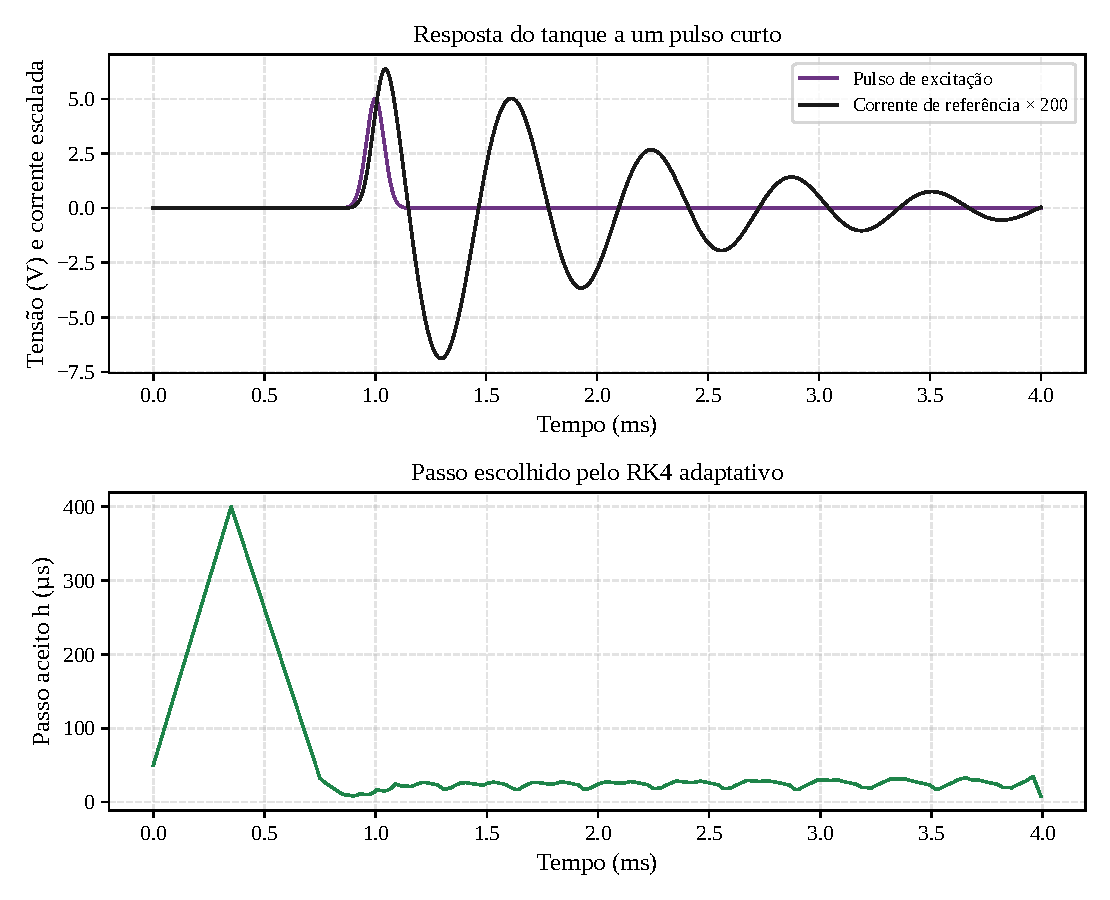
\includegraphics[width=\textwidth]{pulso.pdf}
\fonte{Elaborado pelos autores (2026).}
\end{figure}
